%% LyX 2.5.1 created this file.  For more info, see https://www.lyx.org/.
%% Do not edit unless you really know what you are doing.
\documentclass[10pt,english,t,10pt]{beamer}
\usepackage{lmodern}
\usepackage[T1]{fontenc}
\usepackage[utf8]{inputenc}
\setcounter{tocdepth}{1}
\usepackage{colortbl}
\usepackage{amsbsy}
\usepackage{amstext}
\usepackage{amssymb}
\usepackage{graphicx}
\usepackage[authoryear]{natbib}
\PassOptionsToPackage{normalem}{ulem}
\usepackage{ulem}

\makeatletter

%%%%%%%%%%%%%%%%%%%%%%%%%%%%%% LyX specific LaTeX commands.
%% Because html converters don't know tabularnewline
\providecommand{\tabularnewline}{\\}

%%%%%%%%%%%%%%%%%%%%%%%%%%%%%% Textclass specific LaTeX commands.
% this default might be overridden by plain title style
\newcommand\makebeamertitle{\frame{\maketitle}}%
% (ERT) argument for the TOC
\AtBeginDocument{%
  \let\origtableofcontents=\tableofcontents
  \def\tableofcontents{\@ifnextchar[{\origtableofcontents}{\gobbletableofcontents}}
  \def\gobbletableofcontents#1{\origtableofcontents}
}

%%%%%%%%%%%%%%%%%%%%%%%%%%%%%% User specified LaTeX commands.



\usepackage{tikz}
\usetikzlibrary{positioning}
\usepackage{appendixnumberbeamer}

\usepackage{graphicx}
\usepackage{subfig}

\usetheme[progressbar=frametitle,block=fill,subsectionpage=progressbar]{metropolis}

% margin
\setbeamersize{text margin right=1.5cm}

% colors
\colorlet{DarkRed}{red!70!black}
\setbeamercolor{normal text}{fg=black}
\setbeamercolor{alerted text}{fg=DarkRed}
\setbeamercolor{progress bar}{fg=DarkRed}
\setbeamercolor{button}{bg=DarkRed}

% width of seperators
\makeatletter
\setlength{\metropolis@titleseparator@linewidth}{1pt}
\setlength{\metropolis@progressonsectionpage@linewidth}{1pt}
\setlength{\metropolis@progressinheadfoot@linewidth}{1pt}
\makeatother

% new alert block
\newlength\origleftmargini
\setlength\origleftmargini\leftmargini
\setbeamertemplate{itemize/enumerate body begin}{\setlength{\leftmargini}{4mm}}
\let\oldalertblock\alertblock
\let\oldendalertblock\endalertblock
\def\alertblock{\begingroup \setbeamertemplate{itemize/enumerate body begin}{\setlength{\leftmargini}{\origleftmargini}} \oldalertblock}
\def\endalertblock{\oldendalertblock \endgroup}
\setbeamertemplate{mini frame}{}
\setbeamertemplate{mini frame in current section}{}
\setbeamertemplate{mini frame in current subsection}{}
\setbeamercolor{section in head/foot}{fg=normal text.bg, bg=structure.fg}
\setbeamercolor{subsection in head/foot}{fg=normal text.bg, bg=structure.fg}

% footer
\makeatletter
\setbeamertemplate{footline}{%
    \begin{beamercolorbox}[colsep=1.5pt]{upper separation line head}
    \end{beamercolorbox}
    \begin{beamercolorbox}{section in head/foot}
      \vskip1pt\insertsectionnavigationhorizontal{\paperwidth}{}{\hskip0pt plus1filll \insertframenumber{} / \inserttotalframenumber \hskip2pt}\vskip3pt% 
    \end{beamercolorbox}%
    \begin{beamercolorbox}[colsep=1.5pt]{lower separation line head}
    \end{beamercolorbox}
}
\makeatother

% toc
\setbeamertemplate{section in toc}{\hspace*{1em}\inserttocsectionnumber.~\inserttocsection\par}
\setbeamertemplate{subsection in toc}{\hspace*{2em}\inserttocsectionnumber.\inserttocsubsectionnumber.~\inserttocsubsection\par}
% Added by lyx2lyx
\setlength{\parskip}{\smallskipamount}
\setlength{\parindent}{0pt}

\makeatother

\usepackage{babel}
\begin{document}
\title{13. HANK-SAM\vspace{-2mm}}
\subtitle{Adv. Macro: Heterogenous Agent Models} 
\author{Raphaël Huleux}
\date{2026}

{
\setbeamertemplate{footline}{} 
\begin{frame}

\maketitle

\begin{tikzpicture}[overlay, remember picture]
\node[above left=0cm and 0.0cm of current page.south east] 
{
\includegraphics[width=4cm]{figs/KUSAMFtitlelrcorner.pdf}};
\end{tikzpicture}

\begin{tikzpicture}[overlay, remember picture]
\node[below left=0.5cm and .8cm of current page.north east] 
{\includegraphics[width=1.5cm]{figs/KUSAMFlogo.pdf}};
\end{tikzpicture}

\begin{tikzpicture}[overlay, remember picture]
\node[below right=0.5cm and 0.8cm of current page.north west] 
{
\includegraphics[width=1.5cm]{figs/CEBI.png}};
\end{tikzpicture}

\begin{tikzpicture}[overlay, remember picture]
\node[above right=0.5cm and 0.8cm of current page.south west] 
{
\includegraphics[width=1.5cm]{figs/DNRF.png}};
\end{tikzpicture}

\end{frame}
}

\addtocounter{framenumber}{-1}

\section{Introduction}
\begin{frame}{Introduction}
\vspace{-2mm}
\begin{itemize}
\item \textbf{From RANK to HANK:}
\begin{enumerate}
\item Income effects more important relative to substitution effects
\item Cash-flows more important relative to relative prices
\end{enumerate}
\item \textbf{Central:} High MPCs

{\footnotesize I. Idiosyncratic risk + incomplete markets $\rightarrow$}\\
{\footnotesize II. Precautionary saving and liquidity constraint $\rightarrow$}\\
{\footnotesize III. Concave consumption function $\rightarrow$ high
MPCs}\pause
\item \textbf{SAM:} Search-And-Matching labor market
\item []\textbf{New:} \emph{Endogenous fluctuations in idiosyncratic risk}\pause
\item \textbf{Today: }{\footnotesize}\\
{\footnotesize GEModelTools: Model description of HANK-SAM}\\
{\footnotesize Broer, Druedahl, Harmenberg and Öberg:}\\
{\footnotesize ~~2024: >>Stimulus effects of common fiscal policies<<}\\
{\footnotesize ~~2025: >>The Unemployment-Risk Channel in Business-Cycle
Fluctuations<<}{\footnotesize\par}
\end{itemize}
\end{frame}
%
%

\section{HANK-SAM}
\begin{frame}{Overview}
\begin{itemize}
\item Intermediate \textbf{producers:} 
\begin{enumerate}
\item Hire and fire in search-and-matching labor market
\item Sell homogeneous good at price $p^{X}_{t}$.
\end{enumerate}
\item Wholesale\textbf{ price-setters: }
\begin{enumerate}
\item Set prices in monopolistic competition subject to adjustment costs
\item Pay out dividends
\end{enumerate}
\item Final producers: Aggregate to final good
\item \textbf{Government:}
\begin{enumerate}
\item Pay transfers and unemployment insurance
\item Collect taxes and issues debt
\end{enumerate}
\item \textbf{Central bank:} Sets nominal interest rate
\item \textbf{Households:} Consume and save
\end{itemize}
\end{frame}
%
\begin{frame}{Equilibrium dynamics}
\begin{enumerate}
\item \textbf{Incomplete markets:} Unemployment risk $\rightarrow$ demand

{\footnotesize Complete markets / representative agent:}\\
{\footnotesize Only total income matters}{\footnotesize\par}
\item \textbf{Sticky prices:} Demand $\rightarrow$ profitability
\item \textbf{Frictional labor market:} Profitability $\rightarrow$ unemployment
risk
\end{enumerate}
\end{frame}
%
\begin{frame}{Household problem}

{\footnotesize\vspace{-5mm}}
\begin{align*}
v_{t}(\beta_{i},u_{it},a_{it-1})= & \max_{c_{it},a_{it}}\frac{c^{1-\sigma}_{it}}{1-\sigma}+\beta_{i}\mathbb{E}_{t}\left[v_{t+1}\left(\beta_{i},u_{it+1},a_{it}\right)\right]\\
\text{s.t. } & a_{it}+c_{it}=(1+r_{t})a_{it-1}+(1-\tau_{t})y_{t}(u_{it})+\text{div}_{t}+\text{transfer}_{t}\\
 & a_{it}\geq0
\end{align*}
{\footnotesize\vspace{-7mm}}{\footnotesize\par}
\begin{enumerate}
\item \textbf{Dividends and government transfers:} $\text{div}_{t}$ and
$\text{transfer}_{t}$
\item \textbf{Real wage}: $w_{ss}$
\item \textbf{Income tax: }$\tau_{t}$
\item \textbf{Separation rate} for employed: $\delta_{ss}$
\item \textbf{Job-finding rate }for unemployed: $\lambda^{u,s}_{t}s(u_{it-1})$

{\footnotesize (where $s(u_{it-1})$ is exogenous search effectiveness)}{\footnotesize\par}
\item US-style duration-dependent \textbf{UI system:}\vspace{1mm}

{\footnotesize a) High replacement rate}{\footnotesize\textbf{ $\overline{\phi}$,
}}{\footnotesize first $\overline{u}$ months}{\footnotesize\par}

{\footnotesize b) Low replacement rate }{\footnotesize\textbf{$\underline{\phi}$,}}{\footnotesize{}
after $\overline{u}$ months}{\footnotesize\par}
\end{enumerate}
\end{frame}
%
\begin{frame}{Income process}
\begin{itemize}
\item \textbf{Income} is
\begin{align*}
y_{it}(u_{it}) & =w_{ss}\cdot\begin{cases}
1 & \text{if }u_{it}=0\\
\overline{\phi}\text{UI}_{it}+(1-\text{UI}_{it})\underline{\phi} & \text{else}
\end{cases}
\end{align*}
where the share of the month with UI is
\begin{align*}
\text{UI}_{it} & =\begin{cases}
0 & \text{if }u_{it}=0\\
1 & \text{else }\text{if }u_{it}<\overline{u}\\
0 & \text{else if }u_{it}>\overline{u}+1\\
\overline{u}-\left(u_{it}-1\right) & \text{else}
\end{cases}
\end{align*}
\item \textbf{Note:} \emph{Hereby $\overline{u}$ becomes a continuous variable.}
\end{itemize}
\end{frame}
%
\begin{frame}{Transition probabilities}
\begin{itemize}
\item \textbf{Beginning-of-period value function:}
\[
\underline{v}_{t}\left(\beta_{i},u_{it-1},a_{it-1}\right)=\mathbb{E}\left[v_{t}(\beta_{i},u_{it},a_{it-1})\,|\,u_{it-1},a_{it-1}\right]
\]
\item \textbf{Grid:} $u_{it}\in\{0,1,\dots,\#_{u}-1\}$
\item \textbf{Employed} with $u_{it-1}=0$: $u_{it}=\begin{cases}
0 & \text{with prob. }1-\delta_{ss}\\
1 & \text{with prob. }\delta_{ss}
\end{cases}$
\item \textbf{Unemployed} with $u_{it-1}=1$: 
\[
u_{it}=\begin{cases}
0 & \text{with prob. \ensuremath{\lambda^{u,s}_{t}}}s(u_{it-1})\\
u_{it-1}+1 & \text{with prob. }1-\lambda^{u,s}_{t}s(u_{it-1})
\end{cases}
\]

Trick: $u_{it}=\min\left\{ u_{it-1}+1,\#_{u}-1\right\} $
\item \textbf{All unemployed search: }$s(u_{it-1})=\begin{cases}
0 & \text{if }u_{it-1}=0\\
1 & \text{else}
\end{cases}$ 
\end{itemize}
\end{frame}
%
\begin{frame}{Aggregation}
\begin{itemize}
\item \textbf{Distributions:}
\begin{enumerate}
\item Beginning-of-period: $\underline{\boldsymbol{D}}_{t}$ over $\beta_{i}$,
$u_{it-1}$ and $a_{it-1}$
\item At decision: $\boldsymbol{D}_{t}$ over $\beta_{i}$, $u_{it}$ and
$a_{it-1}$
\end{enumerate}
\item \textbf{Stochastic (time-varying) transition matrix:} $\Pi_{t,z}=\Pi_{z}(\lambda^{u}_{t})$
\item \textbf{Deterministic savings policy matrix:} $\Lambda^{\prime}_{t}$
\item \textbf{Transition steps:}
\begin{align*}
\boldsymbol{D}_{t} & =\Pi^{\prime}_{t,z}\underline{\boldsymbol{D}}_{t}\\
\underline{\boldsymbol{D}}_{t+1} & =\Lambda^{\prime}_{t}\boldsymbol{D}_{t}
\end{align*}
\item \textbf{Searchers:} $S_{t}=\int s(\beta_{i},u_{it-1},a_{it-1})d\underline{\boldsymbol{D}}_{t}$
\item \textbf{Savings:} $A^{hh}_{t}=\int a^{\ast}_{t}(\beta_{i},u_{it},a_{it-1})d\boldsymbol{D}_{t}$
\item \textbf{Consumption:} $C^{hh}_{t}=\int c^{\ast}_{t}(\beta_{i},u_{it},a_{it-1})d\boldsymbol{D}_{t}$
\end{itemize}
\end{frame}
%
\begin{frame}{EGM}
 
\begin{itemize}
\item \textbf{Beginning-of-period value function: 
\begin{align*}
\underline{v}_{a,t}(\beta_{i},u_{it-1},a_{it-1}) & =\mathbb{E}_{t}\left[v_{a,t}(\beta_{i},u_{it},a_{it-1})\right]=\mathbb{E}_{t}\left[(1+r_{t})c^{-\sigma}_{it}\right]
\end{align*}
}
\item \textbf{Endogenous grid method: }Vary $u_{it}$ and $a_{it}$ to find
\begin{align*}
c_{it} & =(\beta\underline{v}_{a,t+1}(\beta_{i},u_{it},a_{it}))^{-\frac{1}{\sigma}}\\
m_{it} & =c_{it}+a_{it}
\end{align*}
\item \textbf{Consumption:} Use linear interpolation to find 
\[
c^{\ast}_{t}(\beta_{i},u_{it},a_{it-1})\text{ with }m_{it}=(1+r_{t})a_{it-1}
\]
\item \textbf{Savings:} $a^{\ast}(u_{it},a_{it-1})=(1+r_{t})a_{it-1}-c^{\ast}_{t}(\beta_{i},u_{it},a_{it-1})$
\end{itemize}
\end{frame}
%
\begin{frame}{Producers: Hiring and firing}
\begin{itemize}
\item \textbf{Job value:}{\small
\begin{align*}
V^{j}_{t} & =p^{X}_{t}Z_{t}-w_{ss}+\beta^{\text{firm}}\mathbb{E}_{t}\left[(1-\delta_{ss})V^{j}_{t+1}\right]
\end{align*}
}{\small\par}
\item \textbf{Vacancy value: }{\small
\begin{align*}
V^{v}_{t} & =-\kappa+\lambda^{v}_{t}V^{j}_{t}+(1-\lambda^{v}_{t})(1-\delta_{ss})\beta^{\text{firm}}\mathbb{E}_{t}\left[V^{v}_{t+1}\right]
\end{align*}
}{\small\par}
\item \textbf{Free entry }implies 
\[
V^{v}_{t}=0
\]
\end{itemize}
\end{frame}
%
\begin{frame}{Labor market dynamics}
\begin{itemize}
\item \textbf{Labor market tightness }is given by
\[
\theta_{t}=\frac{\text{vacancies}_{t}}{\text{searchers}_{t}}=\frac{v_{t}}{S_{t}}
\]
\item \textbf{Cobb-Douglas matching function }
\[
\text{matches}_{t}=AS^{\alpha}_{t}v^{1-\alpha}_{t},\,\,\,\alpha\in(0,1)
\]

implies the job-filling and job-finding rates: 
\begin{align*}
\lambda^{v}_{t} & =\frac{\text{matches}_{t}}{v_{t}}=A\theta^{-\alpha}_{t}\\
\lambda^{u,s}_{t} & =\frac{\text{matches}_{t}}{S_{t}}=A\theta^{1-\alpha}_{t}
\end{align*}

\item \textbf{Law of motion for unemployment:}
\[
u_{t}=u_{t-1}+\delta_{t}(1-u_{t-1})-\lambda^{u,s}_{t}S_{t}
\]
\end{itemize}
\end{frame}
%
\begin{frame}{Price setters}
\begin{itemize}
\item \textbf{Intermediate goods price:} $p^{X}_{t}$
\item Dixit-Stiglitz \textbf{demand curve} $\Rightarrow$\textbf{ Phillips
curve }relating marginal cost, $MC_{t}=p^{x}_{t}$, and \textbf{final
goods price inflation}, $\Pi_{t}=P_{t}/P_{t-1},$
\[
1-\epsilon+\epsilon p^{x}_{t}=\phi\pi_{t}(1+\pi_{t})-\phi\beta^{\text{firm}}\mathbb{E}_{t}\left[\pi_{t+1}(1+\pi_{t+1})\frac{Y_{t+1}}{Y_{t}}\right]
\]
with output $Y_{t}=Z_{t}(1-u_{t})$
\item \textbf{Flexible price limit:} $\phi\rightarrow0$
\item \textbf{Dividends:}
\[
\text{div}_{t}=Y_{t}-w_{t}(1-u_{t})
\]
\end{itemize}
\end{frame}
%
\begin{frame}{Central bank}
\begin{itemize}
\item \textbf{Taylor rule:}
\begin{eqnarray*}
1+i_{t} & = & \left(1+i_{ss}\right)\left(\frac{1+\pi_{t}}{1+\pi_{ss}}\right)^{\delta_{\pi}}
\end{eqnarray*}
\end{itemize}
\end{frame}
%
\begin{frame}{Government}
\begin{itemize}
\item \textbf{Unemployment insurance:} $\Phi_{t}=w_{ss}\left(\overline{\phi}\text{UI}^{hh}_{t}+\underline{\phi}\left(u_{t}-\text{UI}^{hh}_{t}\right)\right)$
\item \textbf{Total expenses:} $X_{t}=\Phi_{t}+G_{t}+\text{transfer}_{t}$
\item \textbf{Total taxes:} $\text{taxes}_{t}=\tau_{t}\left(\Phi_{t}+w_{ss}(1-u_{t})\right)$
\item \textbf{Government budget} is
\[
q_{t}B_{t}=(1+q_{t}\delta_{q})B_{t-1}+X_{t}-\text{taxes}_{t}
\]

Long-term debt: Real payment stream is $1,\delta,\delta^{2},\dots$. 

The real bond price is $q_{t}.$ 
\item \textbf{Tax rule:}{\small
\begin{align*}
\tilde{\tau}_{t} & =\frac{\left(1+q_{t}\delta_{q}\right)B_{t-1}+X_{t}-q_{ss}B_{ss}}{\Phi_{t}+w_{ss}(1-u_{t})}\\
\tau_{t} & =\omega\tilde{\tau}_{t}+(1-\omega)\tau_{ss}
\end{align*}
}{\small\par}
\item \textbf{Transfers:} $\text{transfer}_{t}=-\text{div}_{ss}$
\end{itemize}
\end{frame}
%
\begin{frame}{Financial markets: No arbitrage}
\begin{enumerate}
\item \textbf{Pricing of government debt:}
\[
\frac{1+\delta_{q}q_{t+1}}{q_{t}}=\frac{1+i_{t}}{1+\pi_{t+1}}=1+r_{t+1}
\]
\item \textbf{Ex post real return:}
\[
1+r_{t}=\begin{cases}
\frac{(1+\delta_{q}q_{0})B_{-1}}{A^{hh}_{-1}} & \text{if }t=0\\
\frac{1+i_{t-1}}{1+\pi_{t}} & \text{else}
\end{cases}
\]
\end{enumerate}
\end{frame}
%

\begin{frame}{Market clearing}
\begin{enumerate}
\item Asset market: $A^{hh}_{t}=q_{t}B_{t}$
\item Goods market: $Y_{t}=C^{hh}_{t}+G_{t}$
\end{enumerate}
\textbf{Tip:} \emph{You should be able to verify Walras' law.}
\end{frame}
%
\begin{frame}{Shocks, target, unknowns}
\begin{enumerate}
\item \textbf{Shocks:} $G_{t}$
\item \textbf{Unknowns:} $p^{X}_{t}$, $V^{j}_{t}$, $v_{t}$, $u_{t}$,
$S_{t}$, $\pi_{t}$, $\text{UI}^{\text{guess}}_{t}$
\item \textbf{Targets:}
\begin{enumerate}
\item Error in Job Value
\item Error in Vacancy Value
\item Error in Law-of-Motion for $u_{t}$ 
\item Error in Philips Curve
\item Error in Asset Market Clearing
\item $u_{t}=U^{^{hh}}_{t}=\int1\{u_{it}>0\}d\boldsymbol{D}_{t}$
\item $\text{UI}^{\text{guess}}_{t}=\text{UI}^{^{hh}}_{t}=\int\text{UI}_{it}d\boldsymbol{D}_{t}$
\end{enumerate}
\end{enumerate}
\end{frame}
%
\begin{frame}{Steady State}
\begin{enumerate}
\item \textbf{Zero inflation: }$\pi_{t}=0$
\item \textbf{SAM: }Choose $A$ and $\kappa$ to ensure $\delta_{ss}=0.02$
and $\lambda^{s}_{u,ss}=0.30$ 
\item \textbf{HANK: }Enforce \emph{asset market clearing}
\begin{enumerate}
\item Set $r_{ss}$ 
\item Calculate implied $A^{hh}_{ss}$ 
\item Adjust $G_{ss}$ so $q_{ss}B_{ss}=A^{hh}_{ss}$
\end{enumerate}
\end{enumerate}
\end{frame}
%
\begin{frame}{Calibration}
\begin{enumerate}
\item \textbf{Real interest rate:} $1+r_{t}=1.02^{\frac{1}{12}}$
\item \textbf{Households: $\sigma=2.0$}

30\%: $\beta_{i}=\beta^{\text{HtM}}=0$

60\%: $\beta_{i}=\beta^{\text{BS}}=0.94^{\frac{1}{12}}$

10\%: $\beta_{i}=\beta^{\text{PIH}}=0.975^{\frac{1}{12}}$
\item \textbf{Matching and bargaining: $\alpha=0.60$,} $\theta=0.60$,
$w_{ss}=0.90$
\item \textbf{Producers: }$\beta^{\text{firm}}=0.975^{\frac{1}{12}}$
\item \textbf{Price-setters: }$\epsilon=6$ and $\phi=600$
\item \textbf{Monetary policy: $\phi=1.5$}
\item \textbf{Government:}

Tax: $\tau=0.30$

Debt: $\delta_{q}=1-\frac{1}{36}$ and $\omega=0.05$

UI: $\overline{\phi}=0.70$, $\underline{\phi}=0.40$, and $\overline{u}=6$
\end{enumerate}
\end{frame}
%
\begin{frame}{Steady state analysis}

In \textbf{steady state:}
\begin{enumerate}
\item Look at the consumption functions
\item Look at the distribution of savings
\item Look at how consumption evolves in unemployment
\end{enumerate}
Look at \textbf{household Jacobians
\[
d\boldsymbol{C}=\boldsymbol{M}^{r}d\boldsymbol{r}+\boldsymbol{M}^{\lambda}d\boldsymbol{\lambda^{u,s}}+\boldsymbol{M}^{\tau}d\boldsymbol{\tau}+\boldsymbol{M}^{\Delta}d\boldsymbol{\Delta}
\]
}where $\Delta_{t}=\text{div}_{t}+\text{transfer}_{t}$
\begin{enumerate}
\item Liquidity effects
\item Precautionary saving effects
\end{enumerate}
\end{frame}
%
\begin{frame}{Policy analysis}

\textbf{Shock: }Consider a 1\% shock to government consumption
\[
G_{t}-G_{ss}=0.80^{t}\cdot0.01\cdot G_{ss}
\]

\vspace{-2mm}Look at \textbf{impulse responses }for\textbf{:}

{\footnotesize ~~1. Output}{\footnotesize\par}

{\footnotesize ~~2. Unemployment (risk)}{\footnotesize\par}

{\footnotesize ~~3. Tax rate}{\footnotesize\par}

\textbf{What drives the consumption response?}

{\footnotesize ~~1. Interest rate}{\footnotesize\par}

{\footnotesize ~~2. Tax rate}{\footnotesize\par}

{\footnotesize ~~3. Job-finding rate}{\footnotesize\par}

{\footnotesize ~~4. Dividends}{\footnotesize\par}

\textbf{\emph{Is the effect from the job-finding rate larger than
an equivalent change in income causes by wages? Why?}}

\end{frame}
%

\section{Stimulus Effects of Common Fiscal Policies}
\begin{frame}{Motivation and question}
\begin{itemize}
\item \textbf{Resurgence of countercyclical fiscal policy for stabilization
}\vspace{2mm}
\item \textbf{Often: }What's the size of \emph{\alert{\emph{the}}} fiscal
multiplier to gov. spending?{\footnotesize}\\
{\footnotesize Christiano–Eichenbaum–Rebelo (2011); Ramey (2016); Auclert–Rognlie–Straub
(2024) }\vspace{2mm}
\item In practice, \textbf{policy design varies widely (often transfers)} 
\begin{itemize}
\item \uline{Households}: Cash transfers, UI increases, UI duration extensions 
\item \uline{Firms}: Retention and hiring subsidies \vspace{2mm}
\end{itemize}
\item \alert{\textbf{Research question}}\\
\emph{ Which fiscal transfer policies are most cost effective? }
\end{itemize}
\end{frame}
%
\begin{frame}{A HA-NK-SAM model}
\begin{itemize}
\item []\textbf{HA:} Incomplete asset market
\item []\textbf{NK:} Pricing frictions in the goods market 
\item []\textbf{SAM:} Search frictions in the labor market \vspace{2mm}
\item \textbf{Policy:} 
\begin{itemize}
\item Fiscal authority finances expenditures through taxes and debt
\item Monetary authority follows inflation-targeting Taylor-rule \vspace{2mm}
\end{itemize}
\item \textbf{Calibration:} 
\begin{enumerate}
\item Realistic degree of partial self-insurance 
\begin{itemize}
\item[$\Rightarrow$] Matches micro-level consumption profiles during unemployment 
\end{itemize}
\item Realistic hiring-and-firing dynamics 
\begin{itemize}
\item[$\Rightarrow$] Matches macro-level dynamics of job-finding and separation rates 
\end{itemize}
\end{enumerate}
\end{itemize}
\end{frame}
%
\begin{frame}{Overview}
\begin{itemize}
\item \textbf{Types of fiscal policy:}
\begin{enumerate}
\item Government consumption, $G_{t}$
\item Universal transfer, $T_{t}=\text{transfer}_{t}$
\item Higher unemployment benefits, $\overline{\phi}_{t}$
\item Longer unemployment benefit duration, $\overline{u}_{t}$
\item Hiring subsidies, $hs_{t}$
\item Retention subsidies, $rs_{t}$
\end{enumerate}
\item \textbf{Extended model:}
\begin{enumerate}
\item Endogenous separations + sluggish entry
\item Dividends distributed equally
\item Decreasing search intensity/efficiency while unemployed
\item Risk of no unemployment benefits
\item More detailed calibration
\end{enumerate}
\item \textbf{Previous paper:} Broer et. al. (2025) in zero-liquidity
\end{itemize}
\end{frame}
%
\begin{frame}{Model summary}
\begin{itemize}
\item \textbf{Notation: $\boldsymbol{x}=\left[X_{0}-X_{ss},X_{1}-X_{ss},\dots\right]$}
\item \textbf{Household policies:
\[
\boldsymbol{h}=\left[\boldsymbol{g},\boldsymbol{t},\boldsymbol{\overline{\phi}},\boldsymbol{\overline{u}}\right]'
\]
}
\item \textbf{Firm policies:
\[
\boldsymbol{f}=\left[\boldsymbol{hs},\boldsymbol{rs}\right]'
\]
}
\item \textbf{Income process: 
\[
\boldsymbol{inc}=\left[\boldsymbol{\boldsymbol{\delta}},\boldsymbol{\lambda^{u}},\boldsymbol{div}\right]'
\]
}
\item \textbf{Model summary:}
\begin{align}
\boldsymbol{r^{real}} & =M_{HA}\boldsymbol{inc}+M_{h,r}\boldsymbol{h}+\text{\ensuremath{M_{f,r}\boldsymbol{f}},}\label{eq:HA}\\
\boldsymbol{p^{x}} & =M_{NK}\boldsymbol{r^{real}},\label{eq:NK}\\
\boldsymbol{inc} & \boldsymbol{=}M_{SAM}\boldsymbol{p^{x}}+M_{s,inc}\boldsymbol{f}.\label{eq:SAM}
\end{align}
\end{itemize}
\end{frame}
%
\begin{frame}{Directed Cycle Graph}


\includegraphics[width=1\textwidth]{figs/model_diagram}
\end{frame}
%
\begin{frame}{Directed Cycle Process}

If there is a unique solution to the system \eqref{eq:HA}-\eqref{eq:SAM},
it is given by
\[
\boldsymbol{inc}=\underset{\text{GE}}{\underbrace{\mathcal{G}}}\times\left(\underset{\text{first round, household transfer policy}}{\underbrace{M_{\text{SAM}}M_{\text{NK}}\underset{\text{direct}}{\underbrace{M_{h,r}\boldsymbol{h}}}}}+\underset{\text{first round, firm transfer policy}}{\underbrace{M_{SAM}M_{NK}\underset{\text{direct}}{\underbrace{M_{f,r}\boldsymbol{f}}}+\underset{\text{direct}}{\underbrace{M_{f,\text{inc}}\boldsymbol{f}}}}}\right),
\]
where $\mathcal{G}$ is defined by 
\[
\mathcal{G}=(I-M_{SAM}M_{NK}M_{HA})^{-1}.
\]

\end{frame}
%
\begin{frame}{Fiscal multipliers}
\begin{itemize}
\item \textbf{Fiscal multiplier:}\vspace{-2mm}
\begin{align*}
\mathcal{M} & =\text{cumulative fiscal multiplier}=\frac{\boldsymbol{1}^{\prime}\boldsymbol{y}}{\boldsymbol{1}^{\prime}\boldsymbol{taxes}}.\\
\boldsymbol{taxes} & =M_{\text{inc},\text{taxes}}\boldsymbol{inc}+M_{h,taxes}\boldsymbol{h}
\end{align*}
\item \textbf{Household policies 0 and 1:} If same direct PE real interest
rate
\[
M_{h,r}\boldsymbol{h}^{0}=M_{h,r}\boldsymbol{h}^{1}
\]
then output and income are the same $\boldsymbol{y}^{0}=\boldsymbol{y}^{1}$
and $\boldsymbol{inc}^{0}=\boldsymbol{inc}^{1}$.

Differences in taxes are due to direct fiscal costs
\[
\boldsymbol{1}^{\prime}\boldsymbol{taxes}^{0}-\boldsymbol{1}^{\prime}\boldsymbol{taxes}^{1}=\boldsymbol{1}^{\prime}M_{h,\text{taxes}}\boldsymbol{h}^{0}-\boldsymbol{1}^{\prime}M_{h,\text{taxes}}\boldsymbol{h}^{1},
\]
\textbf{Fiscal multipliers are ordered by direct fiscal costs:}
\[
\mathcal{M}_{h^{0}}\gtreqless\mathcal{M}_{h^{1}}\iff\boldsymbol{1}^{\prime}M_{h,\text{taxes}}\boldsymbol{h}^{0}\lesseqgtr\boldsymbol{1}^{\prime}M_{h,\text{taxes}}\boldsymbol{h}^{1}.
\]

\item \textbf{Firm policies: }Same result, but only with representative
agent
\end{itemize}
\end{frame}
%
\begin{frame}{Policy experiment}
\begin{itemize}
\item \textbf{Experiment:} Same output path for different policies.
\end{itemize}
\begin{center}
\begin{tabular}{cc}
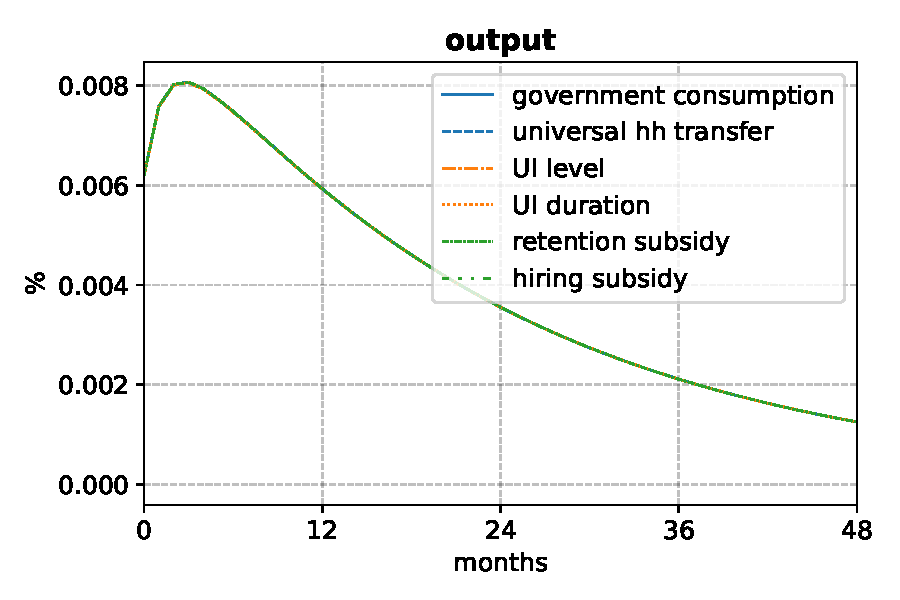
\includegraphics[width=0.5\linewidth]{results/policies_Y_titled} & 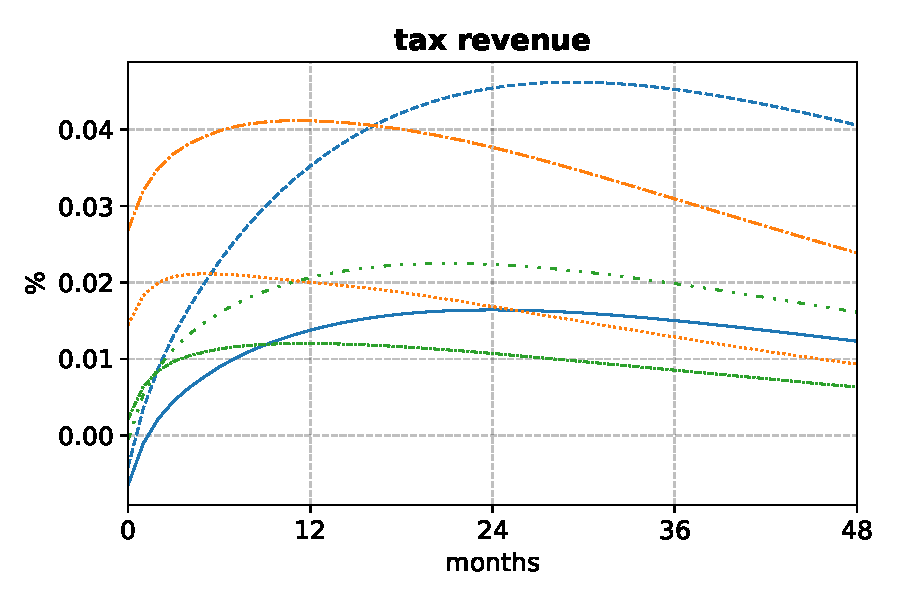
\includegraphics[width=0.5\linewidth]{results/policies_tax_titled}\tabularnewline
\end{tabular}
\par\end{center}

\end{frame}
%
\begin{frame}{Different fiscal multipliers}
\begin{center}
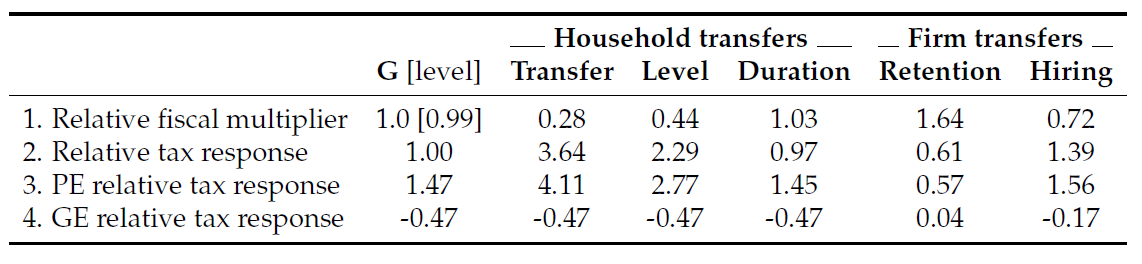
\includegraphics[width=1\textwidth]{figs/table4}
\par\end{center}
\begin{itemize}
\item \textbf{Relative fiscal multiplier:} \textbf{$\frac{\mathcal{M}_{h^{j}}}{\mathcal{M}_{h^{G}}}$}
\item \textbf{Relative tax respones:} \textbf{$\frac{\boldsymbol{1}^{\prime}\boldsymbol{taxes}^{j}}{\boldsymbol{1}^{\prime}\boldsymbol{taxes}^{G}}$}

Decomposition for household transfers:
\begin{align*}
\boldsymbol{taxes}^{j} & =M_{\text{inc},\text{taxes}}\boldsymbol{inc}^{j}+M_{h,taxes}\boldsymbol{h}^{j}\\
\text{\ensuremath{\boldsymbol{taxes}^{j,\text{PE}}}} & =M_{h,\text{taxes}}\boldsymbol{h}^{j}\\
\text{\ensuremath{\boldsymbol{taxes}^{j,\text{GE}}}} & =M_{\text{inc},\text{taxes}}\boldsymbol{inc}^{j}
\end{align*}

\end{itemize}
\end{frame}
%
\begin{frame}{Determinants of fiscal multipliers}
\begin{center}
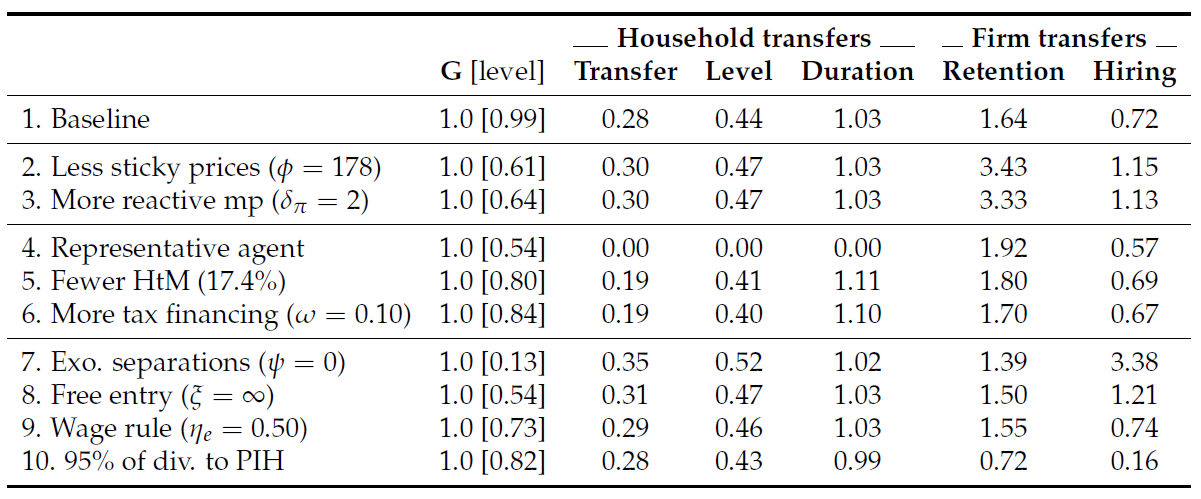
\includegraphics[width=1\textwidth]{figs/table5}
\par\end{center}

\end{frame}
%

\section{Endogenous search{*}}
\begin{frame}{Endogenous search}
\begin{itemize}
\item \textbf{Search decision:}
\begin{enumerate}
\item Discrete search choice:\textbf{ $s_{it}\in\{0,1\}$}
\item Search cost: $\lambda$ if $s_{it}=1$ 
\item Taste shocks: $\varepsilon\left(s_{it}\right)\sim\text{Extreme value}$
(Iskhakov et. al., 2017)
\end{enumerate}
\item \textbf{Note:} Drop $\beta_{i}$ for notational simplicity
\item \textbf{Warning I:} \emph{This is advanced! Only if time permits.}
\item \textbf{Warning II:} \emph{Not implemented in GEModelTools}
\end{itemize}
\end{frame}
%
\begin{frame}{Discrete search decision}
\begin{itemize}
\item \textbf{Search intensity matter for transition:}
\[
\underline{v}_{t}\left(\beta_{i},u_{it-1},a_{it-1}\,|\,s_{it}\right)=\mathbb{E}\left[v_{t}(\beta_{i},u_{it},a_{it-1})\,|\,u_{it-1},a_{it-1},s_{it}\right]
\]
\item \textbf{Standard logit formula:
\begin{align*}
\underline{v}_{t}(u_{it-1},a_{it-1}) & =\max_{s_{it}\in\{0,1\}}\left\{ \underline{v}_{t}(u_{it-1},a_{it-1}\,|\,s_{it})-\lambda\boldsymbol{1}_{s_{it}=1}+\sigma_{\varepsilon}\varepsilon\left(s_{it}\right)\right\} \\
 & =\sigma_{\varepsilon}\log\left(\exp\frac{\underline{v}_{t}(u_{it-1},a_{it-1}\,|\,0)}{\sigma_{\varepsilon}}+\exp\frac{\underline{v}_{t}(u_{it-1},a_{it-1}\,|\,1)}{\sigma_{\varepsilon}}\right)
\end{align*}
}
\end{itemize}
\end{frame}
%
\begin{frame}{Envelope condition}
\begin{itemize}
\item \textbf{Choice probabilities:
\[
P_{t}(s\,|\,u_{it-1},a_{it-1})=\frac{\exp\frac{\underline{v}_{t}(u_{it-1},a_{it-1}\,|\,s)}{\sigma_{\xi}}}{\sum_{s^{\prime}\in\left\{ 0,1\right\} }\exp\frac{\underline{v}_{t}(u_{it-1},a_{it-1}\,|\,s^{\prime})}{\sigma_{\xi}}}
\]
}
\item \textbf{Envelope condition:
\begin{align*}
\underline{v}_{a,t}(u_{t-1},a_{t-1}) & =\sum_{s\in\{0,1\}}P_{t}(s\,|\,u_{it-1},a_{it-1})\pi_{t}(u_{it}\,|\,u_{it-1},s)v_{a,t}(u_{it},a_{it-1})\\
 & =\sum_{s\in\{0,1\}}P_{t}(s\,|\,u_{it-1},a_{it-1})\pi_{t}(u_{it}\,|\,u_{it-1},s)c^{\ast}_{t}(u_{it},a_{it-1})^{-\sigma}
\end{align*}
}
\item \textbf{Break of }\textbf{\emph{monotonicity $\Rightarrow$ }}FOC
still \emph{necessary}, but not \emph{sufficient}
\begin{enumerate}
\item \textbf{Normally:} Savings\textbf{ $\uparrow$ $\Rightarrow$ }future
consumption\textbf{ $\uparrow$ $\Rightarrow$ }marginal utility $\downarrow$
\item \textbf{Now also:} Future search jump $\downarrow$ $\Rightarrow$
future income $\downarrow$ \\
$\Rightarrow$ future consumption $\downarrow$ $\Rightarrow$ marginal
utility $\uparrow$
\end{enumerate}
\end{itemize}
\end{frame}
%
\begin{frame}{Upper envelope for given $z^{i_{z}}$}
\begin{enumerate}
\item \textbf{Generate candidate points:} $\forall i_{a}\in\{0,1,\dots,\#_{a}-1\}$
\begin{align*}
w^{i_{a}} & =\beta\underline{v}_{t+1}(z^{i_{z}},a^{i_{a}})\\
c^{i_{a}} & =u^{\prime-1}\left(\beta\underline{v}_{a,t+1}(z^{i_{z}},a^{i_{a}})\right)\\
m^{i_{a}} & =a^{i_{a}}+c^{i_{a}}\\
v^{i_{a}} & =u\left(c^{i_{a}}\right)+w^{i_{a}}
\end{align*}
\item \textbf{Apply upper-envelope:} $\forall i_{a-}\in\{0,1,\dots,\#_{a}-1\}$
\begin{align*}
c^{\ast}(a^{i_{a-}}) & =\max_{j\in\{0,1,\dots\#_{a}-2\}}u\left(c^{i_{a-}}\right)+w^{i_{a-}}\text{ s.t.}\\
m^{i_{a-}} & =(1+r_{t})a^{i_{a-}}+w_{t}z^{i_{z}}\in\left[m^{j},m^{j+1}\right]\\
c^{i_{a-}} & =\min\left\{ \text{interp }\left\{ m^{i_{a}}\right\} \rightarrow\left\{ c^{i_{a}}\right\} \text{ at }m^{i_{a-}},m^{i_{a-}}\right\} \\
a^{i_{a-}} & =m^{i_{a-}}-c^{i_{a-}}\\
w^{i_{a-}} & =\text{interp }\left\{ a^{i_{a}}\right\} \rightarrow\left\{ w^{i_{a}}\right\} \text{ at }a^{i_{a-}}
\end{align*}
\end{enumerate}
\end{frame}
%
\begin{frame}{Illustration}

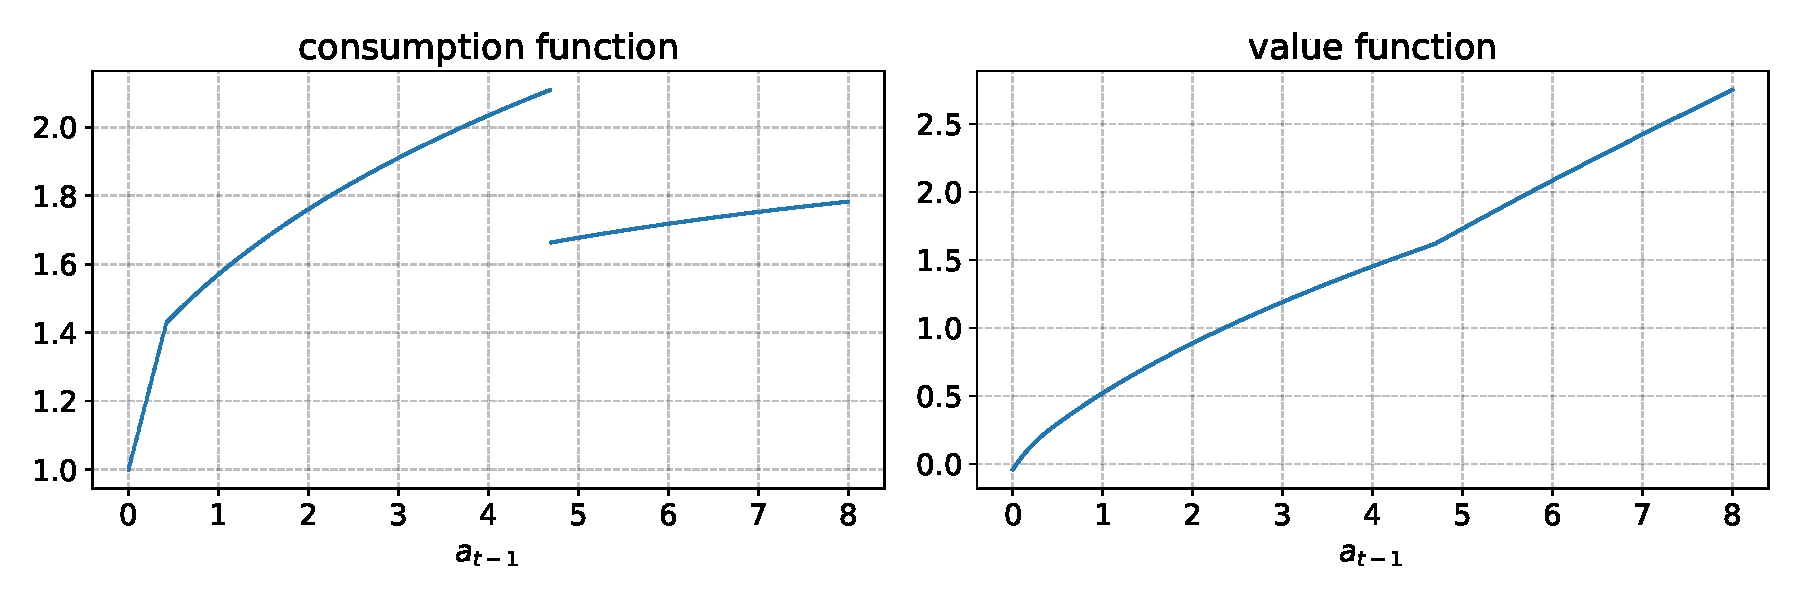
\includegraphics[width=1\textwidth]{figs/upper_envelope}
\begin{enumerate}
\item \vspace{-6mm}\textbf{Numbering:} Different levels of end-of-period
assets, $a^{i_{a}}$
\item \textbf{Problem:} Find the consumption function at $m_{1}$ and $m_{2}$
\item \textbf{Largest value-of-choice:} Denoted by the \emph{triangles}\vspace{1mm}
\end{enumerate}
\textbf{Source:} Druedahl and Jørgensen (2017), $G^{2}EGM$
\end{frame}
%
\begin{frame}{Example}
\begin{itemize}
\item \textbf{Beg.-of-period value function:}
\begin{align*}
\underline{v}_{t+1}(a_{t}) & =\sqrt{m_{t+1}}+\eta\max\left\{ m_{t+1}-\underline{m},0\right\} \\
 & \text{where }m_{t+1}=(1+r)a_{t}+1
\end{align*}
\item \textbf{Derivative:}
\[
\underline{v}_{a,t+1}(a_{t})=\frac{1}{2}(1+r)m^{-\frac{1}{2}}_{t+1}+(1+r)\eta\boldsymbol{1}\left\{ m_{t+1}>\underline{m}\right\} 
\]
\item \textbf{Budget constraint:
\[
a_{t}+c_{t}=(1+r)a_{t-1}+1
\]
}
\end{itemize}
\end{frame}
%
\begin{frame}{Next-period values}

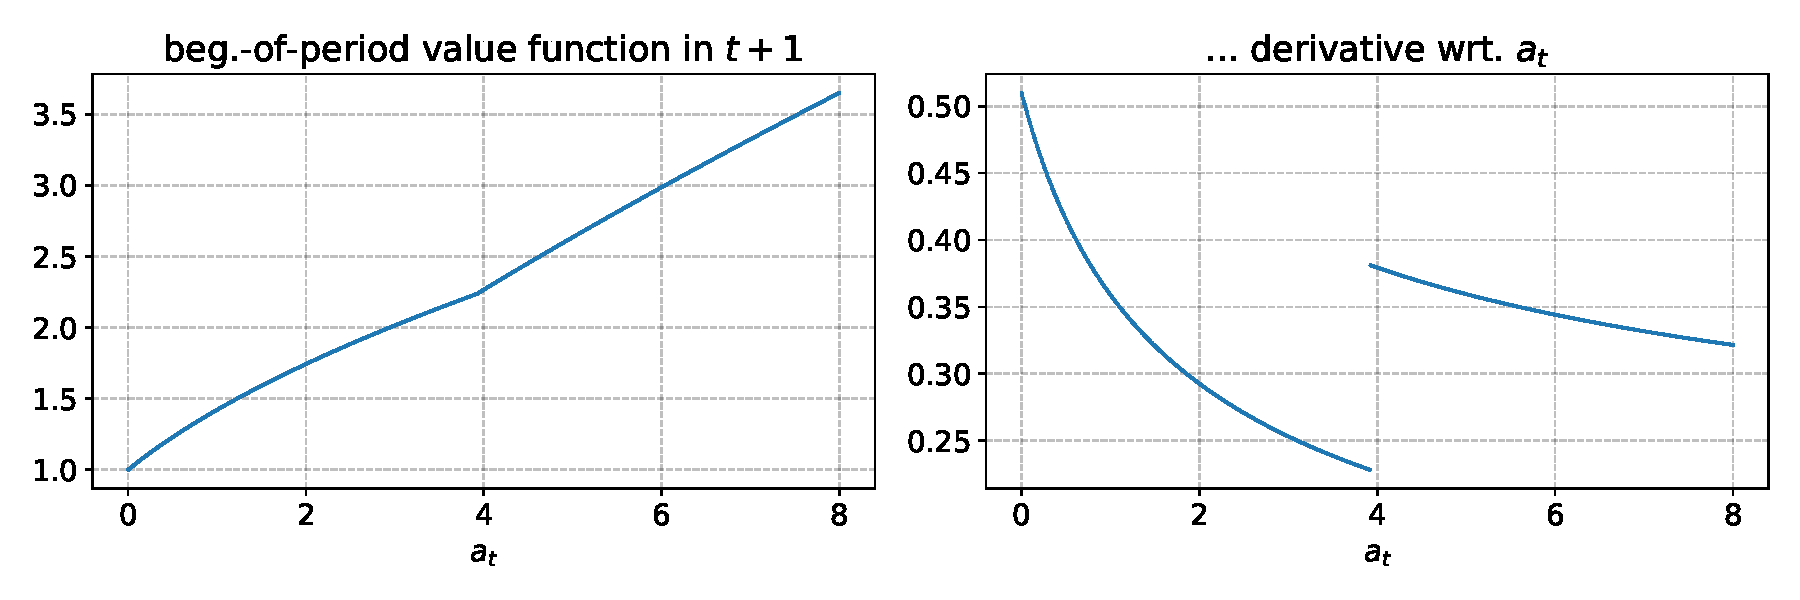
\includegraphics[width=1\textwidth]{figs/upper_envelope_next_period}
\end{frame}
%
\begin{frame}{Raw values of $c^{i_{a}}$ and $v^{i_{a}}$}

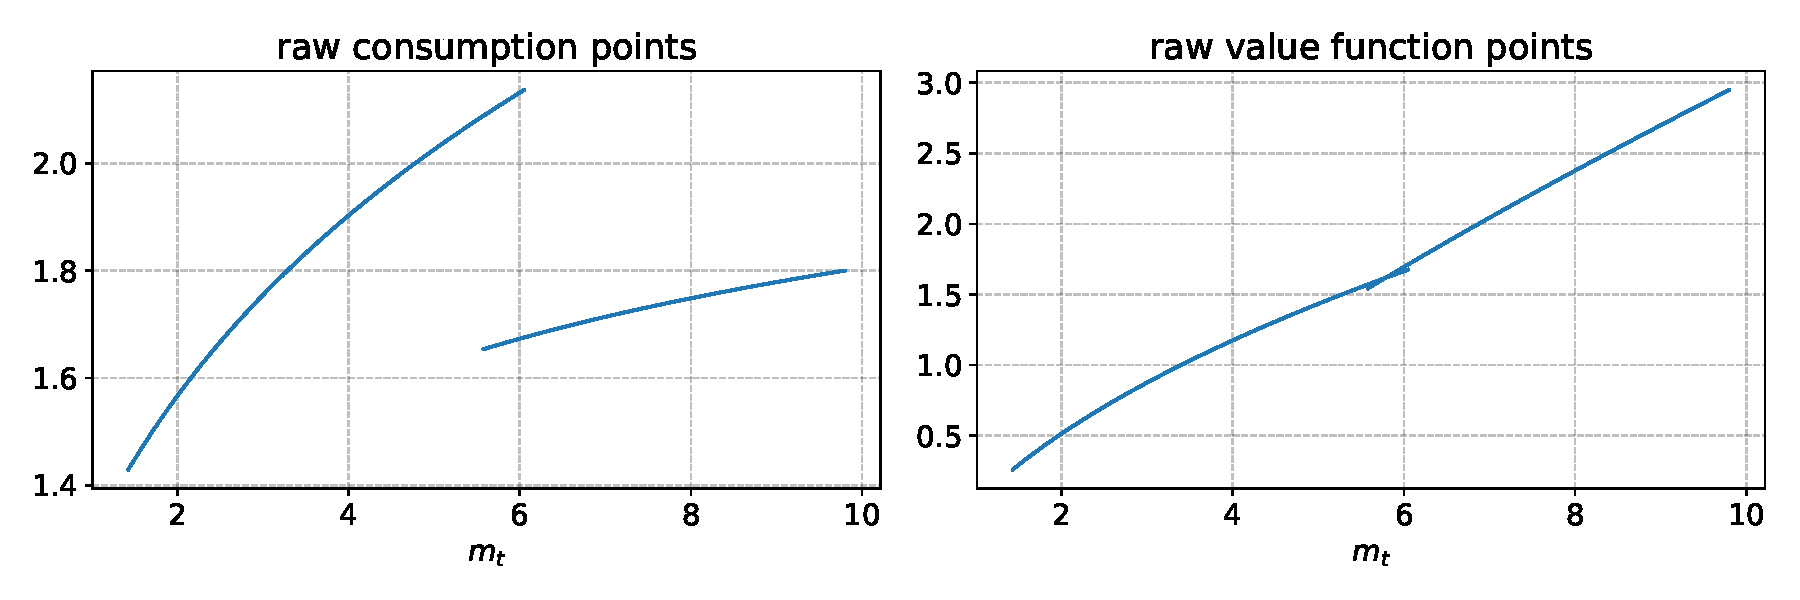
\includegraphics[width=1\textwidth]{figs/upper_envelope_raw}

\textbf{Problem:} Overlaps $\Rightarrow$ not a function $m_{t}$!
\end{frame}
%
\begin{frame}{Result after upper envelope}

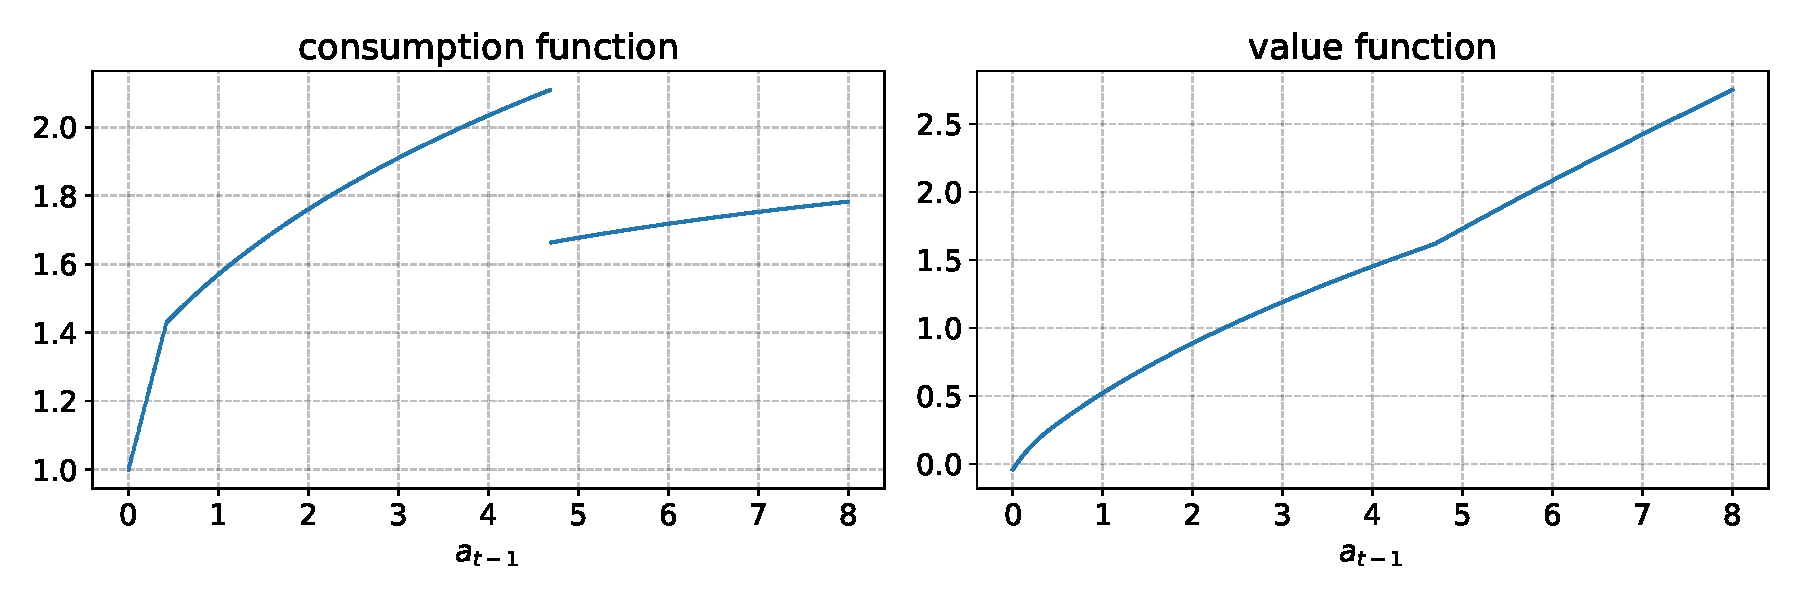
\includegraphics[width=1\textwidth]{figs/upper_envelope}
\end{frame}
%
\begin{frame}{General problem structure}
\begin{itemize}
\item \textbf{General problem structure with }\textbf{\emph{nesting}}\textbf{:}
\begin{align*}
\overline{v}_{t}\left(\overline{x}_{t},d_{t},e_{t},m_{t}\right) & =\max_{c_{t}\in\left[0,m_{t}\right]}u(c_{t},d_{t},e_{t})+\beta\underline{v}_{t+1}\left(\underline{\Gamma}_{t}\left(\overline{x}_{t},d_{t},e_{t},a_{t}\right)\right)\\
 & \text{with }a_{t}=m_{t}-c_{t}\\
v(x_{t}) & =\max_{d_{t}\in\Omega^{d}(x_{t})}\overline{v}_{t}\left(\overline{\Gamma}_{t}\left(x_{t},d_{t}\right)\right)\\
\underline{v}_{t}\left(\underline{x}_{t}\right) & =\max_{e_{t}\in\Omega^{e}(\underline{x}_{t})}\mathbb{E}\left[v\left(\Gamma\left(\underline{x}_{t},e_{t}\right)\right)\,|\,\underline{x}_{t},e_{t}\right]
\end{align*}
\item \textbf{Finding $c_{t}$: }\emph{EGM with upper envelope can (typically)
still be used}
\item \textbf{Finding $d_{t}$ and $e_{t}$:}
\begin{enumerate}
\item Combination of discrete and continuous choices
\item Typically requires use of numerical optimizer or root-finder
\end{enumerate}
\item \textbf{Druedahl (2021),} >>A Guide on Solving Non-Convex Consumption-Saving
Models<< (costly with extra states in $\overline{v}$)
\end{itemize}
\end{frame}
%

\section{Summary}
\begin{frame}{Summary}
\begin{itemize}
\item \textbf{HANK-SAM:}
\begin{enumerate}
\item More realistic labor market and income process
\item Allow for fluctuations in idiosyncratic risk
\item Laboratory for studying e.g. fiscal policy
\end{enumerate}
\item \textbf{Solution methods:}
\begin{enumerate}
\item Time-varying transition matrix is straightforward
\item (Non-sufficient Euler-equation create serious problems)
\end{enumerate}
\end{itemize}
\end{frame}
%

\end{document}
